
%(BEGIN_QUESTION)
% Copyright 2006, Tony R. Kuphaldt, released under the Creative Commons Attribution License (v 1.0)
% This means you may do almost anything with this work of mine, so long as you give me proper credit

The measurement of oxygen content in the exhaust of a combustion heater (or boiler) is very important both for maximizing fuel efficiency and for minimizing pollution (specifically, the production of NO$_{x}$ molecules).  Ideally, a burner's exhaust gas will contain no oxygen, having consumed it all in the process of combustion with a perfect stoichiometric mix of fuel and air.  In practice, the exhaust gas of an efficiently-controlled burner will be somewhere near 2\%, as opposed to the normal 21\% of ambient air.

One way to measure the oxygen content of hot exhaust is to use a {\it high-temperature zirconium oxide} detector.  This detector is made of a ``sandwich'' of platinum electrodes on either side of a solid zirconium oxide electrolyte.  One side of this electrochemical cell is exposed to the exhaust gas (process), while the other side is exposed to heated air which serves as a reference:

$$\includegraphics[width=15.5cm]{i00655x01.eps}$$

Voltage output by the cell is predicted by the Nernst equation:

$$V = {{R T} \over {nF}} \ln \left({C_1 \over C_2}\right)$$

\noindent
Where,

$V$ = Voltage produced across membrane due to ion exchange, in volts (V)

$R$ = Universal gas constant (8.315 J/mol$\cdot$K)

$T$ = Absolute temperature, in Kelvin (K)

$n$ = Number of electrons transferred per ion exchanged (unitless)

$F$ = Faraday constant, in coulombs per mole (96,485 C/mol e$^{-}$)

$C_1$ = Concentration of measured solution, in moles per liter of solution ($M$)

$C_2$ = Concentration of reference solution (on other side of membrane), in moles per liter of solution ($M$)

\vskip 10pt

In order for the cell to function properly, it must be maintained at a high temperature (approximately 800$^{o}$ C).  Accurate measurement and/or control of cell temperature is vital to accurate measurement of oxygen.

\vskip 10pt

Explain why temperature is such a critical factor to the function of this sensor technology, and also characterize the relationship between measured oxygen content and cell output voltage (i.e. is voltage directly or inversely related to oxygen content?).

\underbar{file i00655}
%(END_QUESTION)





%(BEGIN_ANSWER)

The reason why temperature is so critical should be obvious upon inspection of the Nernst equation.  As for oxygen/voltage characterization, let's just say this: the cell output will be zero (0) if the process gas contains just as much oxygen as the reference (air).

%(END_ANSWER)





%(BEGIN_NOTES)


%INDEX% Chemistry, electro-: Nernst equation
%INDEX% Measurement, analytical: oxygen (high temperature)

%(END_NOTES)


